\clearpage\subsection{Vertical Reflection}
A vertical reflection is achieved when $a$ is negative. A negative value for $a$ means every value for a function $f(x)$ that used to be positive becomes negative. For example, when $a = 1$ for the function $f(x) = x$, inputting $x = 1$ produces $y = 1$. However, for a function $g(x) = -x$, where $a = -1$, plugging $x = 1$ produces $y = -1$.
\begin{center}\vspace{-0.25cm}
    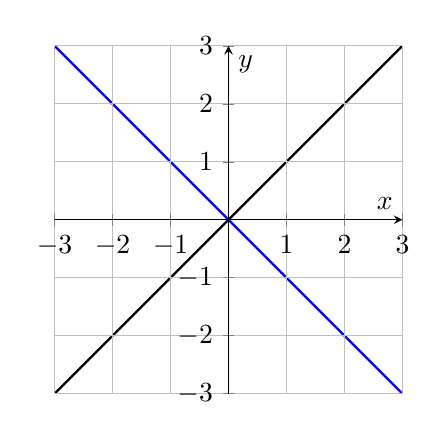
\begin{tikzpicture}
        \begin{axis} [
            axis lines=middle,
            xlabel = $x$, ylabel = {$y$},
            xmin = -3, xmax = 3,
            ymin = -3, ymax = 3,
            xtick distance={1}, ytick distance={1},
            grid = both,
            width = 6cm,
            height = 6cm,
            smooth,
            axis on top
        ]

            \addplot[black, thick, smooth, domain = -3:3, samples = 100]{x};
            \addplot[blue, thick, smooth, domain = -3:3, samples = 100]{-1 * x};
        \end{axis}
    \end{tikzpicture}\\
    $f(x) = x$ (Black), 
    $g(x) = -x$ (Blue),
\end{center}
\begin{definition}
    Given a function $f(x)$, a vertical reflection, also called a reflection along the $x-axis$ or $y = 0$, occurs when $a < 0$. For the function $g(x) = af(x)$, all values in the range are switched from positive to negative (and vice versa), and then stretched by $|a|$.
    \begin{itemize}
        \item When $a < -1$, vertical stretching in the negative direction occurs.
        \item When $-1 < a < 0$, vertical compressing in the negative direciton occurs.
        \item When $a = -1$, the function is reflected without stretching or compressing.
    \end{itemize}
\end{definition}